% !TeX root = ..\..\main.tex
\chapter{Introduction}
\pagenumbering{arabic} %Start roman numbering

This report studies a vital financial derivative in today's markets, namely options. The option market is widely considered a venue for informed trading \cite{black1975,li2021effect,hu2014,chak2004}, that is investors trading with superior knowledge of the probability distribution of share prices, through either access to private information or skillful processing of public information \cite{grossman1975application}. 
\nline
Numerous empirical studies have shown the importance of the option market, reference and examples. The popularity of options in today's market can easily be seen by the exponential growth in their trading volume from when standardized, exchange-traded stock options were first listed in The Chicago Board Options Exchange in 1973 \cite{markham2002financial}, shown in \autoref{C1fig:OptionVolume}. In 2020 option trading volume became higher than the underlying stock volume for the first time ever \cite{yahooOptions}.

\begin{figure}[H]
    \centering
    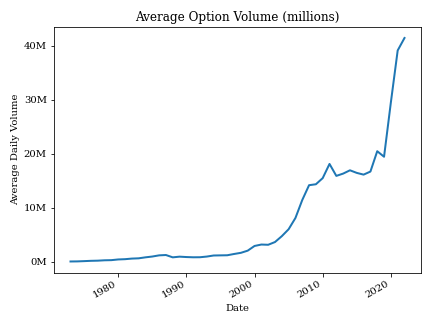
\includegraphics[width=0.65\textwidth]{Chapters/C1/plots/OptionVolume.png}
    \caption{Time series plot of the average daily option and future contracts trading volume per annum. Data provided by the Options Clearing Corporation (OCC) \cite{THEOCC}. Source code \autoref{ApPy:lst option volume plot}}
    \label{C1fig:OptionVolume}
\end{figure}

\section{A brief history of options}



\section{Standard options}

A standard option is a contract between two parties which gives the holder the right to buy (or sell) an asset for an agreed upon (exercise) price prior to, or on a determined (expiry) time in the future; regardless of the current (spot) price. Since the holder of the contract is not obliged to exercise the contract at the expiry time, they would not hold any liability in the absence of a price to purchase the option. The problem then becomes what is the correct price to charge the holder of the option to balance this inequality of liability. 

\section{Asian options}

Whilst standard options, namely European and American style involve using the spot price as the underlying value of the asset; this is not always the case with so-called exotic options. Exotic options differ in their payment structures, expiration dates, and/or strike prices. In the case of exotic fixed-strike price Asian options, the averaging price of the asset is used in place of the underlying asset value. This differs from fixed-price Asian options which instead use the averaging price of the asset to take place of the strike price. These are the two main variations of Asian style options but both of these can be varied further in how the averaging is calculated, for example: geometrically, arithmetically, average taken every day or average taken at the start of each month and so on. They can be varied further by having an expiry structure matching a European or American style option.